\documentclass[10pt]{beamer}
\usepackage{tikz}
\usepackage{tikz-3dplot}
\usetikzlibrary{positioning}
\usepackage{pgfplots}
\usepackage{booktabs}
\usepackage{multirow}
\usepackage{array}
\usepackage{siunitx}
\usepackage{makecell}
\usepackage{CJKutf8}
\usepackage{hyperref}
\usepackage{bookmark}

\pgfplotsset{compat=newest}
\setbeamertemplate{navigation symbols}{}

% Add page number to the lower right corner
\setbeamertemplate{footline}{%
  \hfill\usebeamercolor[fg]{page number in head/foot}%
  \usebeamerfont{page number in head/foot}%
  \insertframenumber\,/\,\inserttotalframenumber\hspace*{1ex}\vskip2pt%
}
\setbeamercolor{page number in head/foot}{fg=gray}
\setbeamerfont{page number in head/foot}{size=\small}

\title{Introduction to Markdown \& LaTeX}
\author{Tzu-You Lin}
\date{May 07, 2025}

% Add this before \begin{document}
\AtBeginSection[]{
  \begin{frame}
    \vfill
    \centering
    \begin{beamercolorbox}[sep=8pt,center,shadow=true,rounded=true]{title}
    \usebeamerfont{title}\insertsectionhead\par%
    \end{beamercolorbox}
    \vfill
  \end{frame}
}

% Add these definitions before \begin{document}
\newcommand{\y}{\mathbf{y}}
\newcommand{\X}{\mathbf{X}}
\renewcommand{\P}{\mathbf{P}}
\newcommand{\M}{\mathbf{M}}
\newcommand{\bvareps}{\boldsymbol{\varepsilon}}

\begin{document}

% Slide 1: Title Page
\begin{frame}[fragile]
    \titlepage
\end{frame}

% Slide 2: Outline
\begin{frame}[fragile]{Outline}
  \tableofcontents
\end{frame}

% --- Section: Markdown ---
\section{Markdown}

% Slide 3: Introduction to Markdown
\begin{frame}[fragile]{What is Markdown?}
  \begin{itemize}
    \item Markdown is a lightweight markup language.
    \item It uses plain text formatting syntax to convert text to HTML (Web pagaes).
    \item Ideal for creating documentation, reports, and readme files.
  \end{itemize}
\end{frame}

% Slide: Markdown Example
\begin{frame}[fragile]{Markdown Example}
    \begin{figure}
        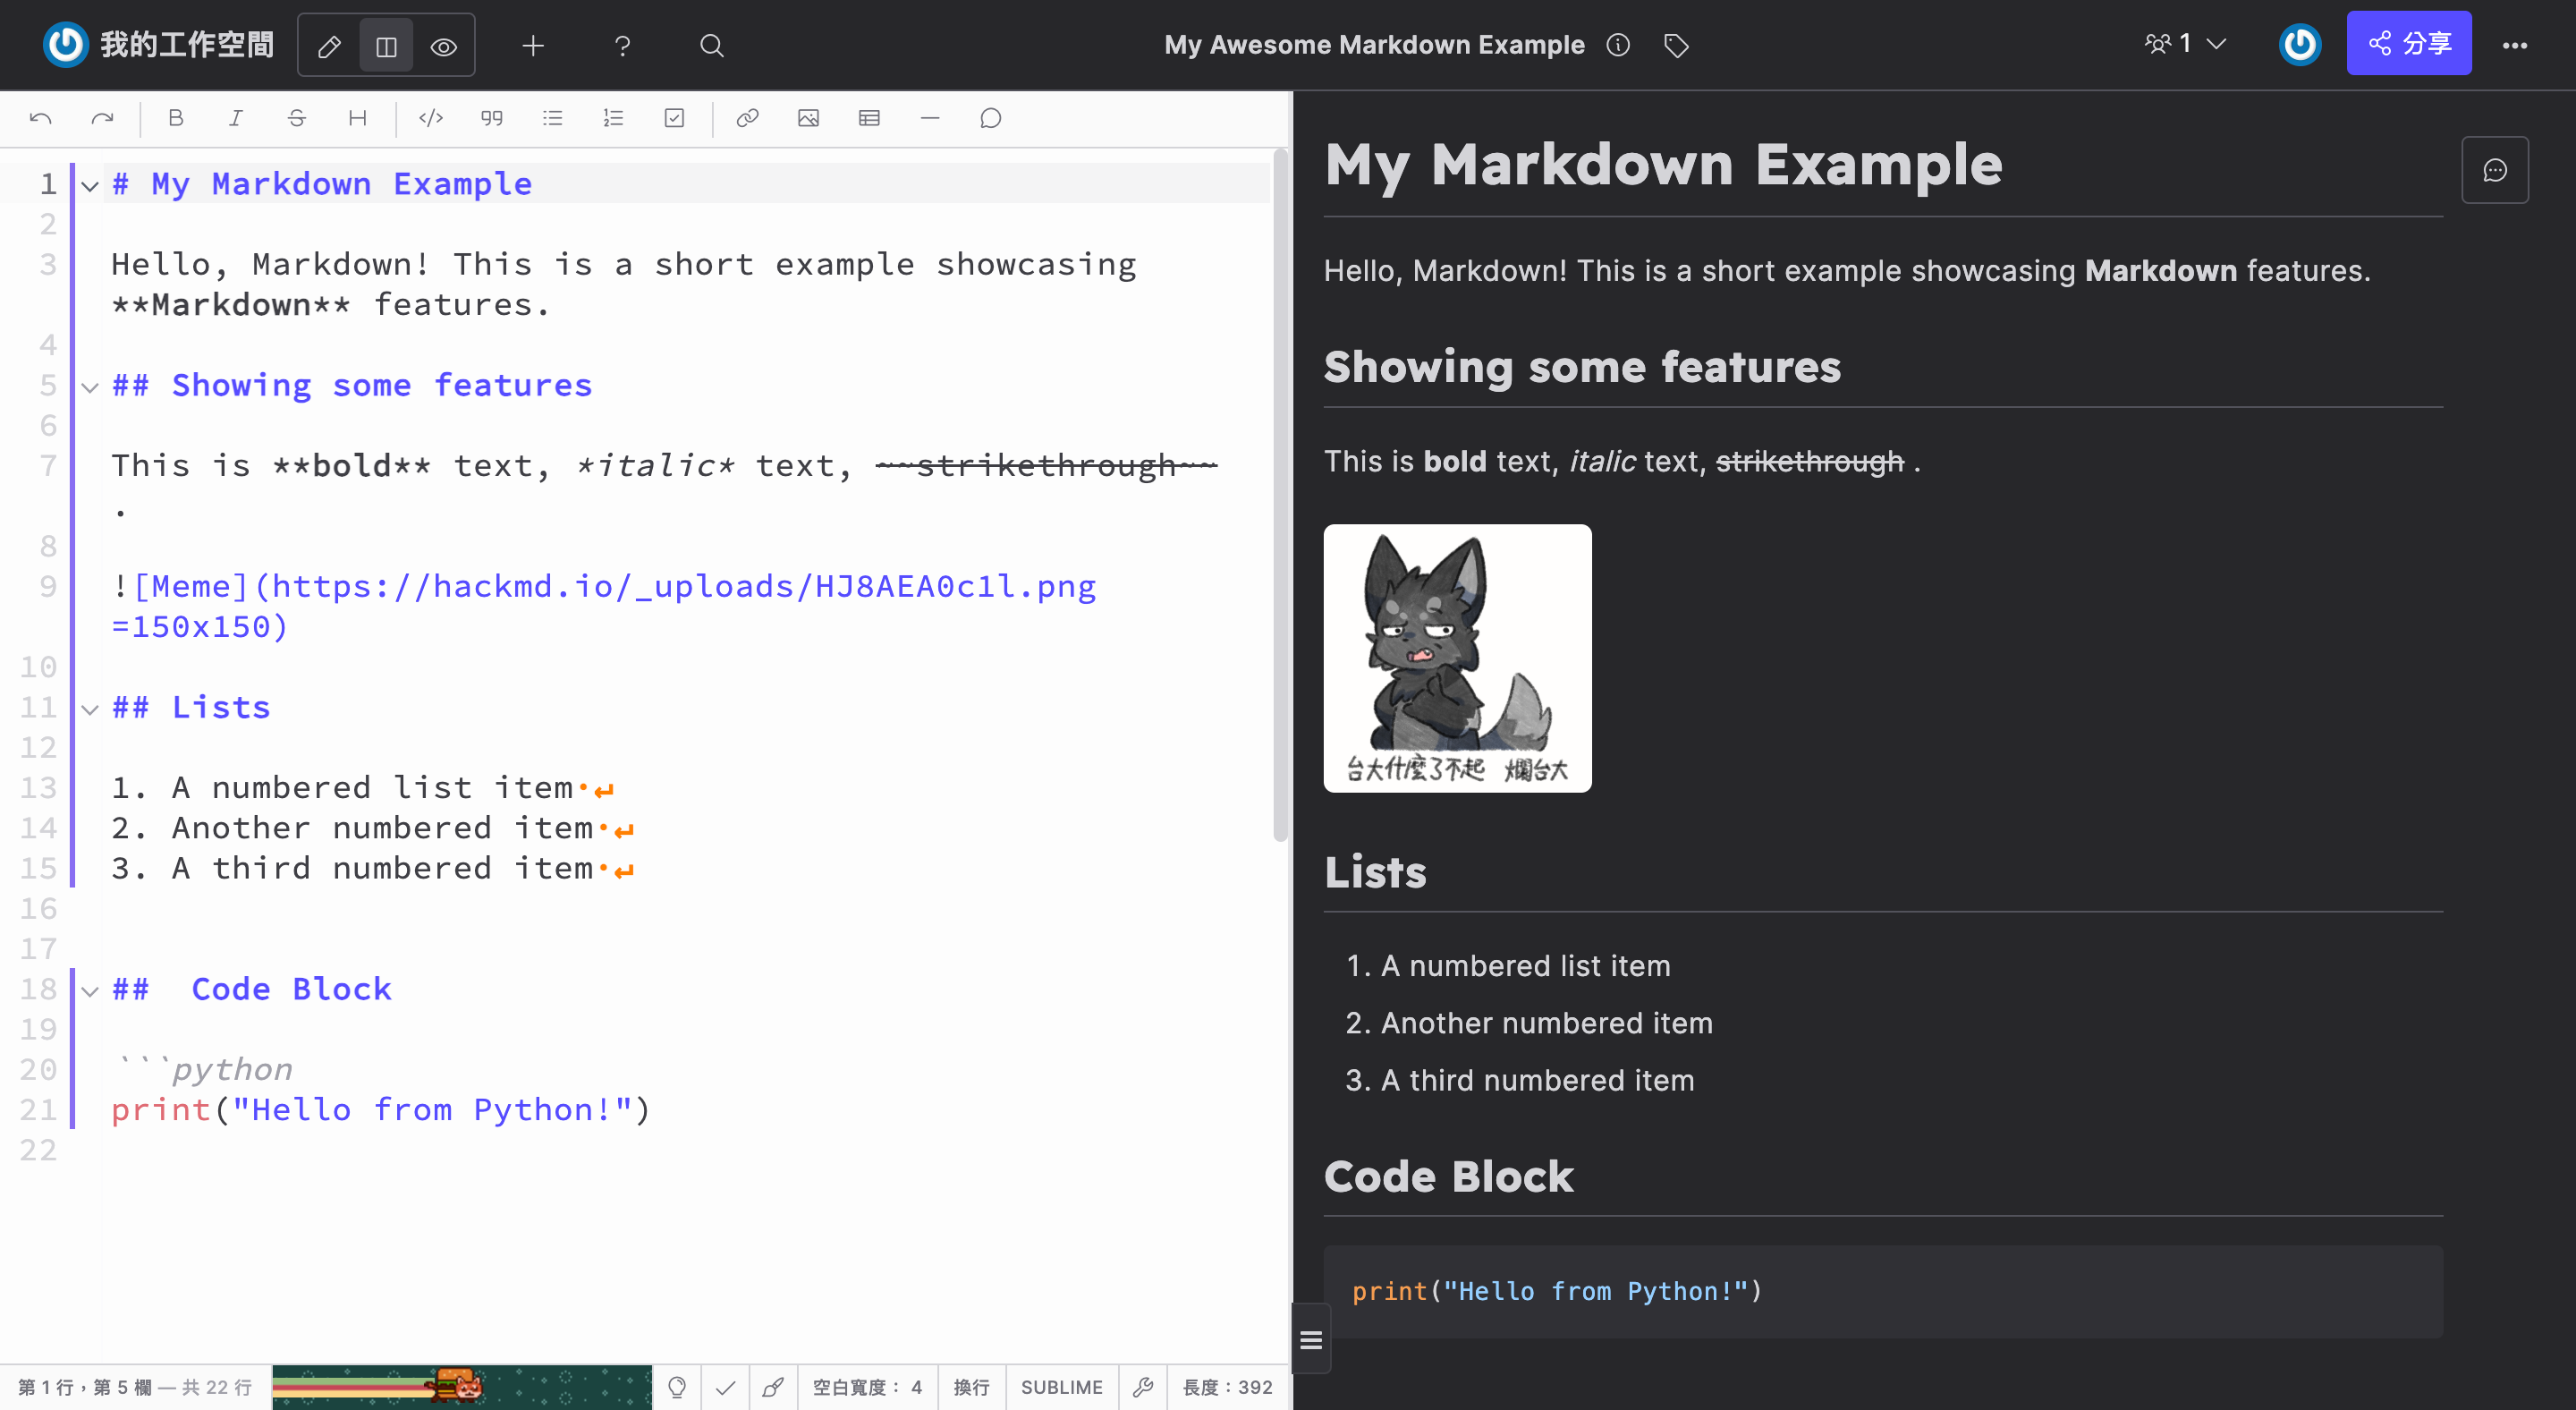
\includegraphics[width=\textwidth]{md_example.png}
        \caption{Example of Markdown formatting and its rendered output}
    \end{figure}
\end{frame}


% Slide 4: Basic Markdown Syntax
\begin{frame}[fragile]{Basic Markdown Syntax}
  \begin{block}{Headers}
    \verb|# Header 1|\\[5pt]
    \verb|## Header 2|\\[5pt]
    \verb|### Header 3|
  \end{block}
  \begin{block}{Emphasis}
    \verb|*italic*| or \verb|_italic_|\\[5pt]
    \verb|**bold**| or \verb|__bold__|
  \end{block}
\end{frame}

% Slide: Tables and TeX in Markdown
\begin{frame}[fragile]{Tables and Math in Markdown}
  \begin{block}{Tables}
    \begin{verbatim}
| Column 1 | Column 2 |
|----------|----------|
| Cell 1   | Cell 2   |
| Cell 3   | Cell 4   |
    \end{verbatim}
  \end{block}
  
  \begin{block}{Math Expressions}
    \begin{itemize}
      \item Inline math: \verb|$E = mc^2$|
      \item Display math: \verb|$$\sum_{i=1}^n x_i = \bar{x}$$|
      \item Supports most LaTeX math syntax
    \end{itemize}
  \end{block}
\end{frame}


% Slide 5: Markdown Code Blocks
\begin{frame}[fragile]{Code Blocks in Markdown}
  \begin{itemize}
    \item Inline code: \verb|`code`|
    \item Multi-line code blocks: Use triple backticks (\verb|```|) before and after the code.
  \end{itemize}
\end{frame}

% Slide 6: Markdown in Econ/DS
\begin{frame}[fragile]{Usage of Markdown}
  \begin{itemize}
    \item Documentation: Clear written explanations of code, methodologies, and project workflows.
    \item Note-taking: Efficient alternative to MS Word for class notes with simple formatting.
    \item Supports structured content with headings, lists, and code examples.
    \item Popular in data science platforms like GitHub, Jupyter Notebooks, and R Markdown for sharing analyses.
    \item Static website generation: Markdown can be used with static site generators like Hexo to create personal blogs and websites (e.g., \url{https://aaronlin1229.github.io/}).
  \end{itemize}
\end{frame}

% Slide: Where to Write Markdown
\begin{frame}[fragile]{Where to Write Markdown \& What to Write}
  \begin{block}{HackMD (\url{https://hackmd.io})}
    \begin{itemize}
      \item Real-time collaborative markdown editor
      \item Perfect for:
        \begin{itemize}
          \item Taking class notes
          \item Writing project documentation
          \item Creating shared meeting notes
        \end{itemize}
    \end{itemize}
  \end{block}

  \begin{block}{Common Document Types}
    \begin{itemize}
      \item README files for code repositories
      \item Technical documentation
      \item Project wikis
      \item Course notes
      \item Blog posts
      \item Quick documentation that needs web rendering
    \end{itemize}
  \end{block}
\end{frame}



% --- Section: LaTeX ---
\section{LaTeX}

% Slide 7: Introduction to LaTeX
\begin{frame}[fragile]{What is LaTeX?}
  \begin{itemize}
    \item LaTeX is the standard typesetting system for writing academic papers and research articles.
    \item It excels at formatting mathematical formulas, tables, figures, and citations needed in papers.
    \item Most academic journals require or strongly prefer LaTeX submissions.
    \item You should notice a lot of your problem sets and tests from other courses are typesetted using LaTeX.
  \end{itemize}

  \vspace{1em}
  \textbf{Benefits:}

  \begin{itemize}
    \item Produces high-quality, publication-ready documents.
    \item Superior handling of equations, tables, and figures.
    \item Ensures consistency in formatting across long documents.
  \end{itemize}
\end{frame}

% Slide 9: Basic LaTeX Document Structure
\begin{frame}[fragile]{Basic LaTeX Structure}
  \begin{block}{Example}
\begin{verbatim}
\documentclass{article}
\begin{document}
Your content here...
\end{document}
\end{verbatim}
  \end{block}
\end{frame}

% Slide 10: Writing Equations
\begin{frame}[fragile]{Writing Equations in LaTeX}
  \begin{block}{LaTeX Code}
    \begin{verbatim}
Inline equation: \( V^{\pi*}(s) \)
Displayed equation:
\[
V^{\pi*}(s)=  \max_a \left\{ {R(s,a) + 
\gamma \sum_{s'} P(s'|s,a) V^{\pi*}(s')} \right\}
\]
    \end{verbatim}
  \end{block}

  \begin{block}{Rendered Output}
    \begin{itemize}
      \item Inline equation: \( V^{\pi*}(s) \)
      \item Displayed equation:
        \[
        V^{\pi*}(s)=  \max_a \left\{ {R(s,a) + \gamma \sum_{s'} P(s'|s,a) V^{\pi*}(s')} \right\}
        \]
    \end{itemize}
  \end{block}
\end{frame}

% Slide 11: Creating Tables
\begin{frame}[fragile]{Creating Tables in LaTeX}
  \begin{block}{LaTeX Code}
    \begin{verbatim}
\begin{tabular}{ccc}
  \toprule
  Variable & Description & Value \\
  \midrule
  \( \alpha \) & Intercept & 0.5 \\
  \( \beta \)  & Slope     & 1.2 \\
  \bottomrule
\end{tabular}
    \end{verbatim}
  \end{block}

  \begin{block}{Rendered Output}
    \begin{center}
      \begin{tabular}{ccc}
        \toprule
        Variable & Description & Value \\
        \midrule
        \( \alpha \) & Intercept & 0.5 \\
        \( \beta \)  & Slope     & 1.2 \\
        \bottomrule
      \end{tabular}
    \end{center}
  \end{block}
\end{frame}

% Slide 13: Including Figures and Plots
\begin{frame}[fragile]{Including Figures and Plots in LaTeX}
  \begin{block}{Example 2D Figure}
    \begin{center}
    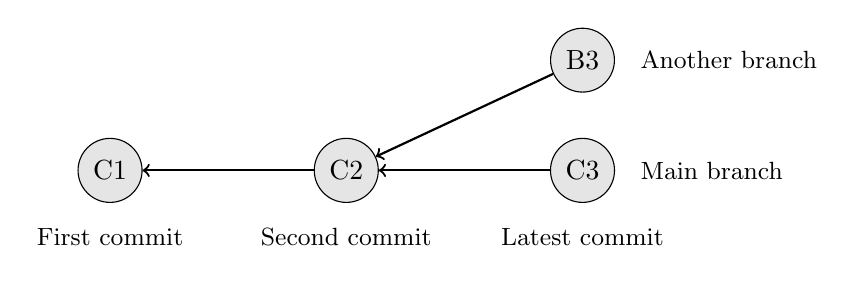
\begin{tikzpicture}[
        commit/.style={circle, draw, fill=gray!20, minimum size=0.75cm},
        arrow/.style={->, thick}
    ]
        \node[commit] (c1) at (0,0) {C1};
        \node[commit] (c2) at (3,0) {C2};
        \node[commit] (c3) at (6,0) {C3};
        \node[commit] (b3) at (6,1.4) {B3};
        
        \draw[arrow] (c2) -- (c1);
        \draw[arrow] (c3) -- (c2);
        \draw[arrow] (b3) -- (c2);
        
        \node[below=0.2cm of c1] {\small First commit};
        \node[below=0.2cm of c2] {\small Second commit};
        \node[below=0.2cm of c3] {\small Latest commit};
        \node[right=0.2cm of b3] {\small Another branch};
        \node[right=0.2cm of c3] {\small Main branch};
    \end{tikzpicture}
    \end{center}
  \end{block}

  \begin{block}{Example 3D Figure}
    \tdplotsetmaincoords{70}{200}
    \begin{center}
    \begin{tikzpicture}[scale = 3,thick,tdplot_main_coords]
    \coordinate (A1) at (0,0,0);
    \coordinate (A2) at (2,0,0);
    \coordinate (A3) at (2,2,0);
    \coordinate (A4) at (0,2,0);

    \coordinate (S) at (0.5,0.5,0);
    \coordinate (E) at (0.5,3,1.5);
    \coordinate (P) at (1.15,1.15,0);
    \fill[fill=blue!20] (A1) -- (A2) -- (A3)  -- (A4) -- cycle;
    \draw[black, -latex] (S) -- (E) node[midway, above] {$\y$};
    \draw[black!80, -latex] (S) -- (P) node[midway, below] {$\hat \y = \mathbf{P} \y$};
    \draw[black!50, dashed, -latex] (P) -- (E) node[midway, left] {$\hat \bvareps = \M \y$};

    \draw[red!70] (2.3,2.3,0.4) node[above] 
    {Column space of $\X$} to [out=-90,in=90] ($(A3)+(-0.2,-0.2,0)$);
    \end{tikzpicture}
    \end{center}
  \end{block}
\end{frame}

% Slide 16: Tools and Platforms
\begin{frame}[fragile]{Where to Write LaTeX?}
  \begin{itemize}
    \item \textbf{Visual Studio Code:} A powerful code editor
      \begin{itemize}
        \item LaTeX Workshop extension
        \item Live preview
        \item Git integration
        \item Customizable environment
      \end{itemize}
    \item \textbf{Overleaf:} An online LaTeX editor
      \begin{itemize}
        \item No setup required
        \item Real-time collaboration
        \item Built-in templates
        \item Access anywhere
      \end{itemize}
    \item \textbf{Key Benefits:}
      \begin{itemize}
        \item VSCode: More control and offline work
        \item Overleaf: Easier to start and collaborate
        \item Both support PDF compilation
      \end{itemize}
  \end{itemize}
\end{frame}

% Slide 17: Practical Tips
\begin{frame}[fragile]{Practical Tips for Beginners}
  \begin{itemize}
    \item Start with simple documents and gradually add complexity
      \begin{itemize}
        \item Begin with basic text and sections
        \item Add equations and tables as needed
        \item Learn advanced features gradually
      \end{itemize}
    \item Use templates available online
      \begin{itemize}
        \item Journal article templates
        \item Presentation templates
        \item Thesis templates
      \end{itemize}
    \item Practice by typesetting your written homework to LaTeX.
    \item Practice typing math equations by: \url{https://texnique.xyz/}
  \end{itemize}
\end{frame}

% Slide 18: Resources and Further Reading
\begin{frame}[fragile]{Resources and Further Reading}
  \begin{itemize}
    \item \textbf{Markdown Guide:} \url{https://www.markdownguide.org}
    \item \textbf{LaTeX Project:} \url{https://www.latex-project.org}
    \item \textbf{Overleaf:} \url{https://www.overleaf.com}
    \item Additional tutorials and documentation are available online
  \end{itemize}
\end{frame}

% Slide 19: Summary
\begin{frame}[fragile]{Summary}
  \begin{itemize}
    \item Markdown offers a simple syntax for quick documentation to be rendered on the web.
    \item LaTeX is a powerful tool for producing professional, technical documents (especially PDF format).
  \end{itemize}
\end{frame}

\end{document}
